





\documentclass[conference]{IEEEtran}
%
\ifCLASSINFOpdf
  
  % \DeclareGraphicsExtensions{.pdf,.jpeg,.png}
\else
  % or other class option (dvipsone, dvipdf, if not using dvips). graphicx
  % will default to the driver specified in the system graphics.cfg if no
  % driver is specified.
  % \usepackage[dvips]{graphicx}
  % declare the path(s) where your graphic files are
  % \graphicspath{{../eps/}}
  % and their extensions so you won't have to specify these with
  % every instance of \includegraphics
  % \DeclareGraphicsExtensions{.eps}
\fi






% correct bad hyphenation here
\hyphenation{op-tical net-works semi-conduc-tor}
\usepackage{listings}

\usepackage{xcolor}
\usepackage{graphicx}
\graphicspath{ {./images/} }

\usepackage{multirow}


\definecolor{codegreen}{rgb}{0,0.6,0}
\definecolor{codegray}{rgb}{0.5,0.5,0.5}
\definecolor{codepurple}{rgb}{0.58,0,0.82}
\definecolor{backcolour}{rgb}{0.95,0.95,0.92}

\lstdefinestyle{mystyle}{
    backgroundcolor=\color{backcolour},   
    commentstyle=\color{codegreen},
    keywordstyle=\color{magenta},
    numberstyle=\tiny\color{codegray},
    stringstyle=\color{codepurple},
    basicstyle=\ttfamily\footnotesize,
    breakatwhitespace=false,         
    breaklines=true,                 
    captionpos=b,                    
    keepspaces=true,                 
    numbers=left,                    
    numbersep=5pt,                  
    showspaces=false,                
    showstringspaces=false,
    showtabs=false,                  
    tabsize=2
}

\usepackage{color}

\definecolor{mygreen}{rgb}{0,0.6,0}
\definecolor{mygray}{rgb}{0.5,0.5,0.5}
\definecolor{mymauve}{rgb}{0.58,0,0.82}

\lstset{ 
  backgroundcolor=\color{white},   % choose the background color; you must add \usepackage{color} or \usepackage{xcolor}; should come as last argument
  basicstyle=\footnotesize,        % the size of the fonts that are used for the code
  breakatwhitespace=false,         % sets if automatic breaks should only happen at whitespace
  breaklines=true,                 % sets automatic line breaking
  captionpos=b,                    % sets the caption-position to bottom
  commentstyle=\color{mygreen},    % comment style
  deletekeywords={...},            % if you want to delete keywords from the given language
  escapeinside={\%*}{*)},          % if you want to add LaTeX within your code
  extendedchars=true,              % lets you use non-ASCII characters; for 8-bits encodings only, does not work with UTF-8
  frame=single,	                   % adds a frame around the code
  keepspaces=true,                 % keeps spaces in text, useful for keeping indentation of code (possibly needs columns=flexible)
  keywordstyle=\color{blue},       % keyword style
  language=Octave,                 % the language of the code
  morekeywords={*,...},            % if you want to add more keywords to the set
  numbersep=5pt,                   % how far the line-numbers are from the code
  numberstyle=\tiny\color{mygray}, % the style that is used for the line-numbers
  rulecolor=\color{black},         % if not set, the frame-color may be changed on line-breaks within not-black text (e.g. comments (green here))
  showspaces=false,                % show spaces everywhere adding particular underscores; it overrides 'showstringspaces'
  showstringspaces=false,          % underline spaces within strings only
  showtabs=false,                  % show tabs within strings adding particular underscores
  stepnumber=2,                    % the step between two line-numbers. If it's 1, each line will be numbered
  stringstyle=\color{mymauve},     % string literal style
  tabsize=2,	                   % sets default tabsize to 2 spaces
  title=\lstname                   % show the filename of files included with \lstinputlisting; also try caption instead of title
}

\lstdefinestyle{customc}{
  belowcaptionskip=1\baselineskip,
  breaklines=true,
  frame=L,
  xleftmargin=\parindent,
  language=C,
  showstringspaces=false,
  basicstyle=\footnotesize\ttfamily,
  keywordstyle=\bfseries\color{green!40!black},
  commentstyle=\itshape\color{purple!40!black},
  identifierstyle=\color{blue},
  stringstyle=\color{orange},
}

\lstdefinestyle{customasm}{
  belowcaptionskip=1\baselineskip,
  frame=L,
  xleftmargin=\parindent,
  language=[x86masm]Assembler,
  basicstyle=\footnotesize\ttfamily,
  commentstyle=\itshape\color{purple!40!black},
}

\lstset{escapechar=@,style=customc}



\providecommand{\keywords}[1]
{
  \small	
  \textbf{\textit{Keywords---}} #1
}



\begin{document}
%
% paper title

\title{Implement KNN Classifier for Sequence Prediction}


% author names and affiliations
% use a multiple column layout for up to three different
% affiliations
\author{\IEEEauthorblockN{Muhammad Haris}
\IEEEauthorblockA{Information Technology (M.Eng.)\\Computer Science and Engineering\\
Frankfurt University of Applied Sciences\\
Frankfurt am Main, Germany\\
Email: Muhammad.Haris@fra-uas.de}
\and
\IEEEauthorblockN{Zaka Ahmed}
\IEEEauthorblockA{Information Technology (M.Eng.)\\Computer Science and Engineering\\
Frankfurt University of Applied Sciences\\
Frankfurt am Main, Germany\\
zaka.ahmed@stud.fra-uas.de}}




% make the title area
\maketitle

% As a general rule, do not put math, special symbols or citations
% in the abstract
\begin{abstract}
Machine learning comes out as an advanced and significant technology, evolving in our daily life. The focus of Machine Learning is to enable computers to learn from the data and make predictions or decisions based on that data, enabling informed decision making without the need of extra instruction or explicit programming for the system to perform task better. The sectors in which machine learning is involved include education, telecommunication, retail, research and development, finance, healthcare, and transportation through data-driven insights. Machine leaning has three basic types: Supervised Leaning, Unsupervised Learning and Reinforcement leaning. In the domain of supervised machine learning, a variety of classifiers abound, including decision trees, support vector machines, Naive Bayes, and K-nearest neighbors (KNN), each tailored to address specific data analysis challenges. Among the numerous machines leaning algorithms, K-Nearest Neighbors (KNN) classifier is simplest and most effective for classification problem. This paper presents the implementation of the k-nearest neighbor (KNN) machine learning algorithm for predicting outcome variables based on input variables. Leveraging the capabilities of Hierarchical Temporal Memory (HTM) for learning complex temporal patterns, our study focuses on predicting types of sequences: even number sequences, odd number sequences, and decimal number sequences. We integrate the KNN model with the Neocortex API to efficiently classify sequences. The KNN model receives input data in the form of Sparse Distributed Representations (SDR) from HTM. We construct a dataset comprising multiple sequence SDRs, each with varying values within a defined threshold. The KNN model processes a stream of sequence SDRs, with the dataset split into 70\% training data and 30\% testing data. During testing, the model accurately classifies sequences, achieving a 90.9\% accuracy rate with some SDR testing data, and consistently predicts matches with 100\% accuracy in most cases. The paper discusses the KNN design procedure, challenges encountered, and potential enhancements to further improve model accuracy.






\end{abstract}\hspace{10pt}

\keywords{Machine Learning, Hierarchical Temporal Memory, K-Nearest Neighbors, Sequence Classification, Integration, Neocortex API, Accuracy Enhancement}





\IEEEpeerreviewmaketitle



\section{Introduction}

\subsection{Background}
KNN was first developed by Joseph Hodges and Evelyn Fix in the year 1951[1] where the further development and we can say the modification are lead by Thomas Cover[2], in statistics the concept of k-nearest neighbors algorithm(k-NN) is involved in the non-parametric supervised learning method. KNN is commonly used for regression and classification. The input is consist of K-neighbour training example in both regression and classification. Remember the output depends on whether the use case is either regression or classification of K-NN. 

\subsection{Regression}
The main difference between classification and regression is that in regression, the output which we get it will become the the object's property value. The value is the sum of the nearest neighbor's values averaged together. If k=1, the output is assigned from that particular single nearest neighbor. 

\subsection{Classification}
The primary difference between the classifier and regression outputs is that in the former case, the output is the class membership. In classification, the object is classified based on the votes of its nearest neighbors. If k = 1, then the object will be in the class of that single nearest neighbor. The simple function of the kNN model is to predict the target class label. In other words, the class label is often described as a majority voting. The most common terms are technically considered "plurality voting" and "majority vote" The term "majority voting" means the majority needs to be greater the 50\%  
for making decisions. The classification problems with only two classes, like binary predictions, there is always a majority. A majority vote is also automatically a plurality vote. We don't require multi-class settings to make predictions via kNN in multi-class settings. 




\section{Methods}

This section includes multiple subsections including description of KNN in detail, second section try to focus on Theoretical background of including how the values determined accuracy and complexity  of the classifier. In the last section of this section is regarding Hierarchical temporal Memory(HTM). 



\subsection{Literature Review}
The K-Nearest Neighbors (KNN) algorithm is a widely-used non-parametric classification method in machine learning. KNN rely on instance-based learning, in which the similarity of newly added data points to previously labeled data points is used to make predictions. In finance, KNN is used for credit scoring, stock analysis and fraud detection. In healthcare sector, KNN is used for patient health monitoring and drug suggestions. If, I will talk about marketing professionally KNN is used as product suggestion, market trend analysis and customer ads suggestions. In most cases KNN is used for determining the specific patterns and tasks like face recognition or image classification. 

Researchers have proposed various enhancements to the traditional KNN algorithm which can improve the scalability and performance. The weight adjustment algorithm is proposed by Han EH., proposed assigning weights to the nearest neighbors based on their distance from the respective point.[11][8]. The assigned weights desgunish, how much the weights influence the classification method. In this way, high weights will be assigned to the one who are closer neigbors, so it give more priority to the similar instances while performing classification.  This technique is usefull where the dataset has many feature, some of which can be considered as unneccessary but it has high cost in context of computational cost.

Zhang et al. has proposed to adjust the value of K based on the local density of data points [3]. This adaptive KNN algorithm dynamically selects the optimal value of K for each query point, leading to more robust predictions. And shows that the adaptive algorithm outperforms many other traditional KNN algorithms. The other approach can be locally adoptive KNN algorithm. It choices the optimal value of K for classifying an input by analyzing the outcomes of cross-validation computations within the local neighborhood of the unlabeled data point.[12]  The approach defined by Song Yang, is to introduce two input parameters. As we know determining the correct value of K depends on the characteristics of the dataset, the selection of correct parmeter for various applications is a challenge. Song Yang suggest to introduce a novel metric that assesses the informativeness of objects to be classified, with informativeness quantifying the significance of data points. 
Two parameter will be K and I as a input. The class is determined based on the majority class of the most informative training examples.[10]

Whereas on the some has proposed to integrated KNN with dimensionality reduction methods such as principal component analysis (PCA) to improve computational efficiency [5]. This a combination is a example of hybrid approach. Whereas other have combined KNN with ensemble methods such as random forests to enhance predictive accuracy [6]. These hybrid approaches enhance the performance as compared to standalone KNN. 








\subsection{K-Nearest Neighbors Parameters and Matrix}
The K-nearest was first used by US Air force to execute characteristics analysis. There are differnet paramenters in KNN classsifier which plays a important role in algorithm designs including distance matrics, K-Value selection, and voting. 




\subsubsection{\textbf{Computing Distance Matrix}}
If we try to revise, k-nearest neighbor algorithm main objective is the identification of the nearest neighbors around the input. The step will be giving a label or name class to that specific point. The first thing is determining the distance metrics. In order to find which class(data point) is nearest to the input data, to do so we will calculate the distance between the data points and query point. We get assistance to decide in which regions the input point belongs. The distance metrics can be either Manhattan distance or any other approach. The first thing is to identify the k-nearest neighbors and then amount of its k-neatest neighbors.The most famous techniques are discussed below:  


\paragraph{\textbf{Euclidean distance (p=2)}}
In the early 300 Era before, mathematician of Greek introduced Euclid while finding the difference between distance and angle. Still Euclid is most common used of distance. From that early, till yet Euclid is widely and applies in two or three dimensions space. The main method, is the root of square distances between two coordinates of a pair of objects. Then there is a square root of the sum of squares of the differences between the corresponding values. [45]

As from the fig.1 we have the 
\begin{math}
(x_1,y_1), and (x_2,y_2)
\end{math}
from we can see that 
\begin{math}
(x_1,x_2), and (y_1,y_2)
\end{math}
are allocated into the two dimensional space. And If we try to build a right angled triangle and draw a hypotenuse straight line between two points(d). The other two sides of a right angle triangle are base and altitude which will be
\begin{math}
|x_1 - y_1|, and |x_1 - y_1|
\end{math}
. So there the hypotenuse(d) is our Euclidean distance which is the between (x1, x2) and (y1, y2). As this is only a straight line so we will use Pythagorean theorem. The distance between 
\begin{math}
(x_1,x_2), and (y_1,y_2)
\end{math}
would be \begin{math}
(x_1,y_1)^2, and (x_2,y_2)^2
\end{math}.
Moreover to find the Euclidean distance between,
\begin{math}
y_n ,  and x_n
\end{math}
the Euclidean distance is
\begin{math}
(x_n - y_n)^2
\end{math} in n-dimensional space. 

\


\begin{math}
Euclidean distance = d(x,y)=\sqrt{\sum_{i=1}^{n} (y_{i} - x_{i})^2}
\newline
\end{math}

\begin{itemize}
    \item \begin{math}
y_{i}
\end{math}
are the coordinates of one point.
\item \begin{math}
x_{i}
\end{math}
are the coordinates of another point.

\item 
d is the distance between
\begin{math}
(x_{1},y_{1}), and, (x_{2},y_{2})
\end{math}

\end{itemize}

Euclidean is limited to real-valued vectors and is most commonly used for distance measures. The straight line between the input point and the other point under measurement is found using the expression above. 


\begin{figure}
    \centering
    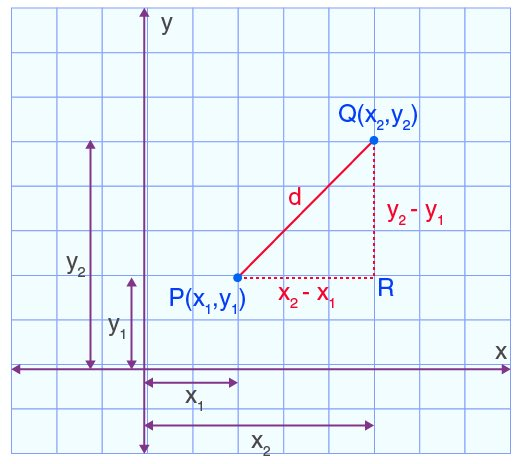
\includegraphics[width=0.7\linewidth]{EDistance.jpg}
    \caption{Euclidean Distance[50]}
    \label{fig:enter-label}
\end{figure}


Euclidean distance is the shortest distance between two points means the straight line between source and destination whereas the Manhattan distance is the sum of all the real distances between the source and destination. And each always be a straight line. The reason behind Euclidean distance used in KNN is that it provides a simple and intuitive measure of similarity between data points in a multi-dimensional space. One of the main reason is that Euclidean distance in KNN, is its computational efficiency and simplicity.[45] Euclidean distance metric works well for continues features and is suitable for data represented in a high-dimensional space. 



Euclidean Distance is largely used in machine learning learning algorithms such as K-Nearest(KNN) where it is used to measure the similarity between two data points.Spatial Analysis for measuring distance between geographical locations.[45] As well as, in robotics for obstacle avoidance and path planning. It is also used in image process for comparing images based on pixel values. Due to coordinate system, making it robust to transformations of the data. It is most widely adopted approach in machine learning applications. 

\



\paragraph{\textbf{Manhattan distance (p=1)}}
In Manhattan distance, the absolute value is measured between two points. Manhattan is widely used as for resolving the problems related to geometry. We can say it as a ordinary distance between two points. Manhattan distance is also one of the popular and dominant distance metrics. The most common example is Uber app visualization with a grid and navigation via streets from one address to another illustration. Manhattan is widely used in cluster analysis. K-Means clustering algorithm is the common example where Manhattan distance is used.[46] The second name of Manhattan Distance is city Block Distance. The easiest method to figure out the distance is to move from one point to the other between two locations by moving horizontally and then vertically, rather than straight forward.[46][56]It only need to subtract instead of performing complicated calculations that why its one of the simplest method of calculating the distance. 

\

\begin{math}
 Manhattan distance = d(x,y)=\sqrt{(\sum_{i=1}^{m} |X_{i} - Y_{i})|)}
 \newline
\end{math}

\
As shown[56], it is the root of squared difference between the coordinates of two objects. We only need to subtract two points instead of performing complex tasks. 

\begin{figure}
    \centering
    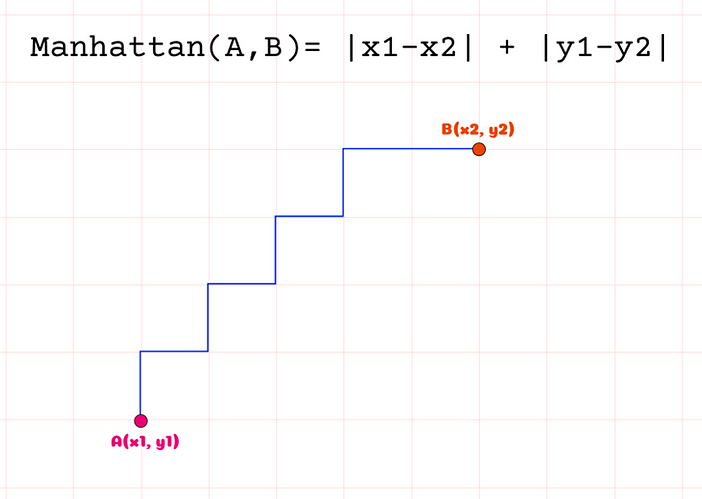
\includegraphics[width=0.8\linewidth]{a.png}
    \caption{Manhattan Distance[49]}
    \label{fig:enter-label}
\end{figure}

\

\paragraph{\textbf{Minkowski distance}}
It is the extrapolate form of Manhattan and Euclidean distance matrices. Manhattan distance is denoted by p equal to one whereas the Euclidean distance is represented by p equal to two[47][56]. Parameter p allows the creation of other distance metrics as shown below.

\begin{math}
 Minkowski distance =\sqrt{(\sum_{i=1}^{n} |X_{i} - Y_{i})|)^1/p}
 \newline
\end{math}

\begin{figure}
    \centering
    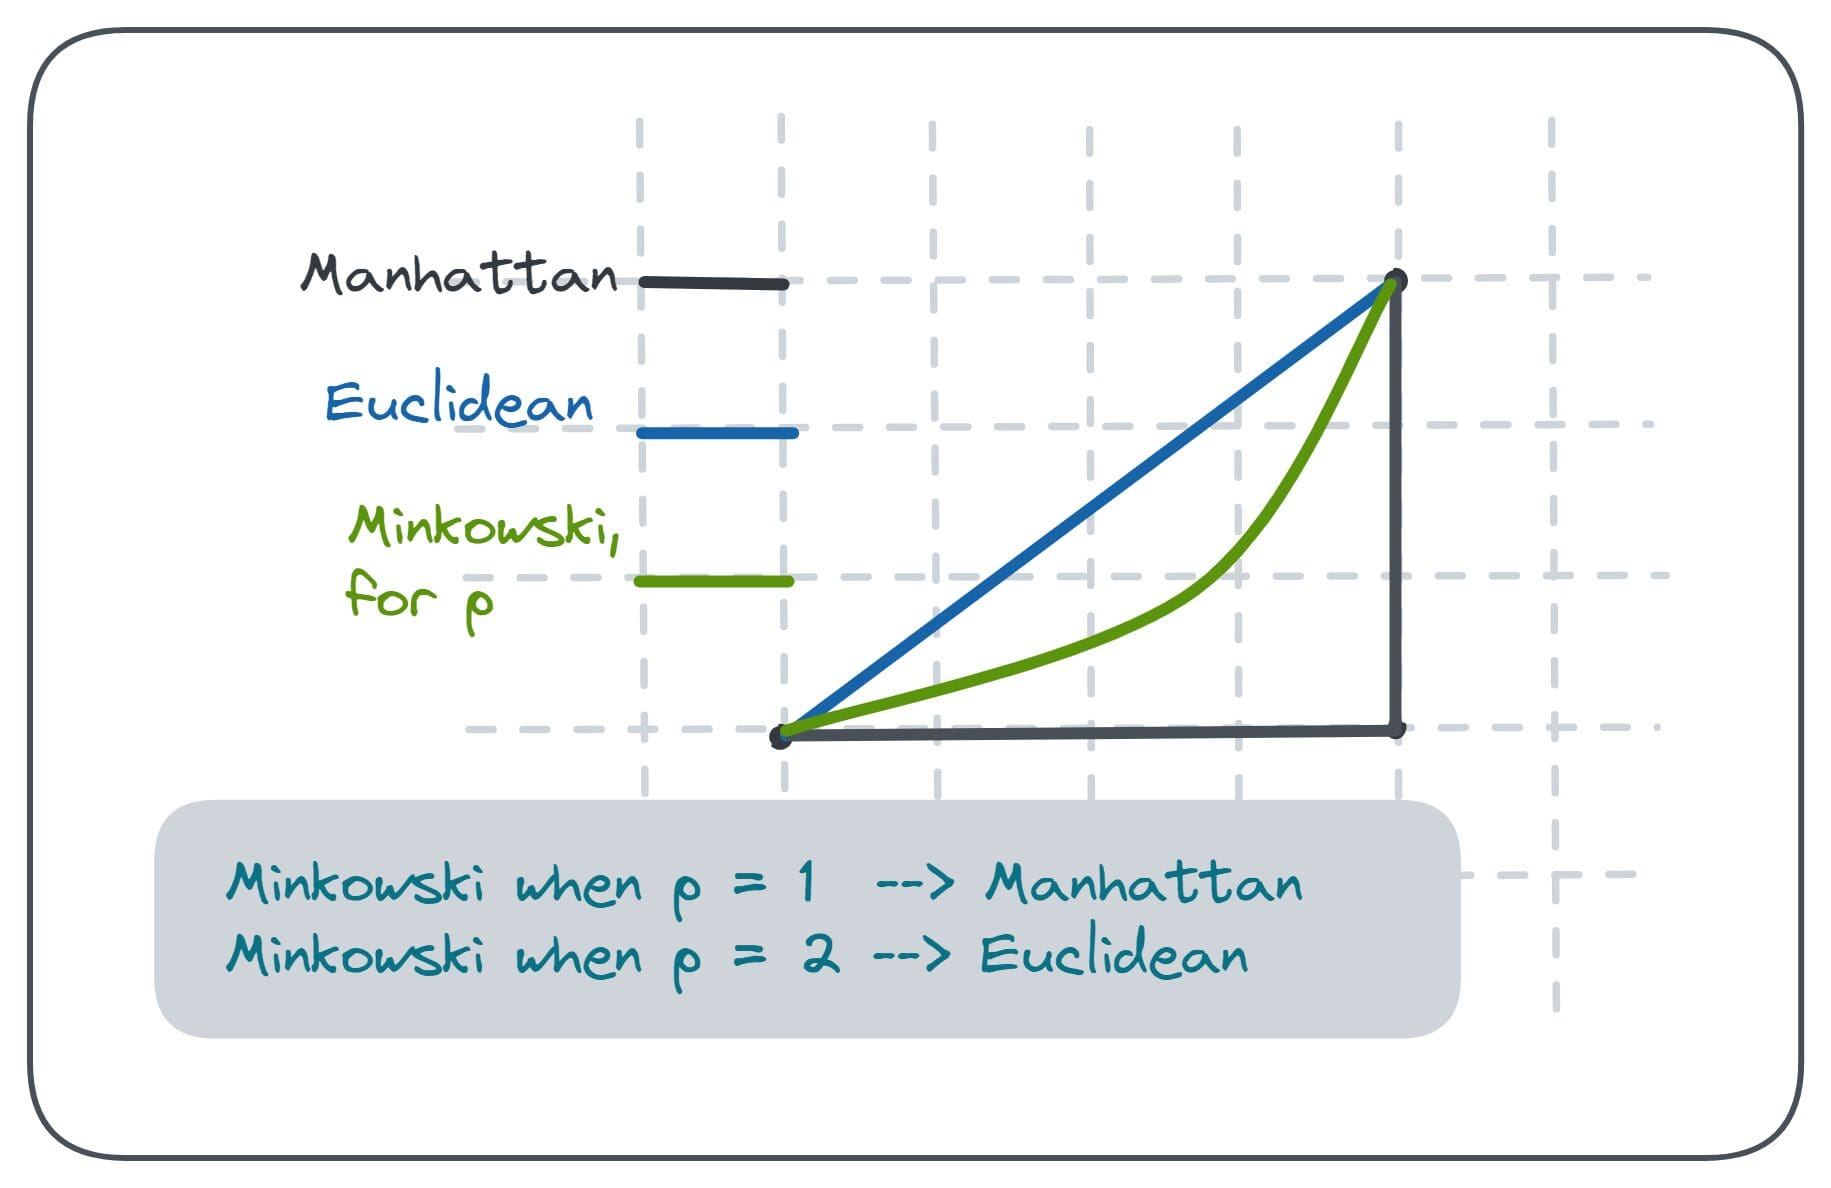
\includegraphics[width=0.8\linewidth]{b.jpg}
    \caption{Difference Between Distance Methods[48]}
    \label{fig:enter-label}
\end{figure}

\paragraph{\textbf{Hamming distance}}
This technique used with string vectors or boolean identifying the points where the vectors do not match.[55] Overlap metrics are also referred as represented below:

\begin{math}
 Hamming Distance = D_{H}=(\sum_{i=1}^{k} |X_{i} - Y_{i})|)
 \newline
\end{math}



\subsubsection{Defining k selection}
In simple words, k is the number of neighbors used for making prediction. The k value indicates how many neighbors will be compared or we can say checked to determine the resultant class in KNN Algorithm. For-example: By changing the value of k the classification can lead to under-fitting or over-fitting. If k=1, the instance will be assigned to the same class because we have a single neighbor. By using lower value of k can low bias, but high variance. As well as, larger value of k may lead to lower variance and high bias.[56] So, we can define k as the balancing act as different values impact the variance on under-fitting or over-fitting. For avoiding ties in classification, k is recommended to be a odd number. The best approach to get a optimal k for you dataset is cross-validation tactics.  


\subsubsection{Voting Principle}
In the KNN algorithm, the prediction is based on the number of K nearest neighbours is considered. The predicted or winning class is determined using the majority voting principle, the class which has high numbers of vote is the class from where our element belongs to. The highest frequency among the K nearest neighbors is chosen. However, the important thing that it is essential to recognize that the choice of K can impact the voting outcome. The higher value of K may leads to less confident predictions.[3][1][2] The scenarios where we have imbalanced data, where one class is higher or outweighs the other class, the majority voting principle can be biased. To resolve such kind of issue techniques like distance-weighted voting and weighted voting us introduced which can help to balance the influence of each class. 

Mathematically, if 
\begin{math}
(C_1,C_2,C_3,.....C_n) 
\end{math}
represent the unique class labels among the K nearest neighbors, and 
\begin{math}
Count(C_i) 
\end{math}
represents the count of occurrences of class 
\begin{math}C_i\end{math}
the predicted class  
\begin{math} y \end{math}
for the new observation is determined by:

\begin{math} y = argmax Count(C_i) 
\end{math}


Where \begin{math} y\end{math} is the predicted class Label.This voting equation ensures that the predicted class is the one that is most prevalent among the K nearest neighbors.Techniques like normalization, standardization, and scaling play a crucial role in preparing the data for modeling in pre-processing.[56] Normalization involves scaling the features to a similar range, typically between 0 and 1, the main advantage of normalization is that it prevents larger scales from dominating the model. Scaling adjusts the range of features to a desired range, which can enhance the performance of algorithms sensitive to feature magnitudes.

As the process diagram (Fig:4) shown the step-by-step procedure, we have adopted in the implementation. In the first step, we feed the input sequences from the text file (3.1) and that specific sequence get encoded. Then after spatial pooler we get sequence SDRs. Then it will be stored in HTM. The next step will be implementation of KNN classifier in which the test data will be mapped, the KNN helps to predict the class from where the sequence blogs to that specific class. The sudo-code of voting is also discussed in the implementation part of paper. 





\begin{figure}
    \centering
    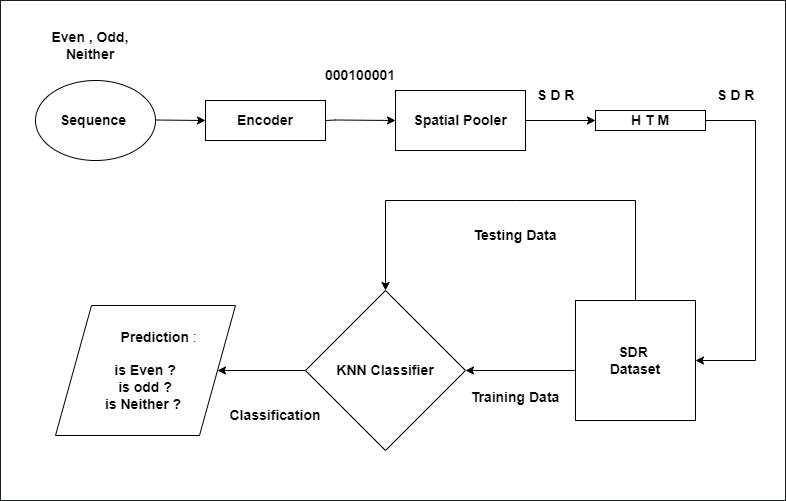
\includegraphics[width=1.0\linewidth]{Process Diagram.png}
    \caption{Process Diagram}
    \label{fig:enter-label}
\end{figure}



\subsection{Overview of HTM}
As the objective behind the HTM CLA is to make a progress towards making a program that functions cognitive tasks as like a simple human being brain. The prediction is done by making a system which can memorize as well as learn from the information executions which are fed before. HTM to anticipate and memorize, it requires user Input. 

As the overall HTM have multiple sections which includes data, Encoder, HTM spatial Pooler, HTM temporal Memory, and HTM Classifier[51]. The data or which is also know as input is a scalar value, data or time, or a picture. Then the next element is encoder which is responsible for changing the data into SDR which can further be used with HTM classifier. SDR is in the cluster of binary input either '0' or '1'. As discussed earlier, input of encoder can be anything a scalar value. It includes locations, weeks, months, time or days in a week etc. 

The next part of the HTM is a spatial pooler it, is an algorithm which learns spatial patterns. The spatial pooler gets an input of bits cluster and converts it into SDR. Next Parts is Temporal memory, it a part which learns the arrangements of SDRs shaped by the spatial pooler algorithm. [51]  


\subsection{Spatial Pooler}
Spatial Poolar is the second phase of HTM learning. It uses the output of the encoder to learn the SDR of the given input binary array. The idea for the spatial poolar SDR is to generate SDRs of the input which is the output of the encoder.[51][52] Once the input SDR are learned, if the same input is given again, it tries to match already learned SDRs and then generates a similar matching SDR.In this method, it will disgunish, is it a same input which is already memorized or a different one.   


\begin{figure}[h]
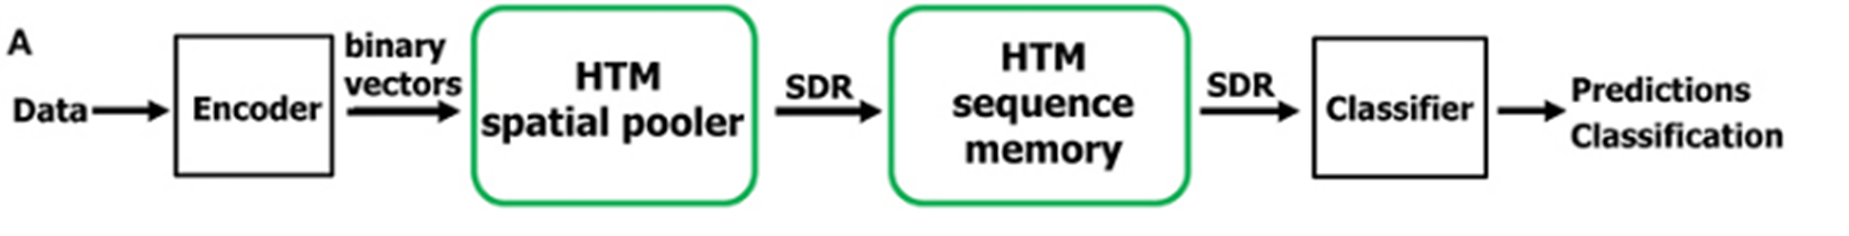
\includegraphics[scale=.40]{HtmPipeline.png}
\caption{General Flow}
\label{fig:enter-label}
\end{figure}






\section{Implementation Details}
The KNN method is divided into two classes first and main class is classifier which is consist of distnace, vote and classify. Second class for indexanddistance. Distance method which is used to calculate the distance of a new data point that has unlabeled data. The voting method is used to prepare the voting table from the distance matrix and the Classify method is used to classify the class of the unknown label data as an output. Remember we are using text file as our dataset which is slit into two parts training and test dataset. As these details are discussed in the further section in details. 


\subsection{Training and Test Dataset}
In the start, we have started with intilizing a array for the data matrix. But later-on we have created a text file from where we read the training data and test dataset. We have divided the file in such a way that 70\% of data act as a training data and other 30\% data in text file act as a test dataset. The large data sets, the technique is not scale able, due to fact that k-NN classifier store all the training data into memory. The below is example of our text file data. 
\begin{lstlisting}
04, 9697, 9772, 9841, 9851, 9922,........, 0
06, 9732, 9753, 9854, 9955, 10107,......., 0
10295, 10353, 10461, 10598, 10612,......., 1
06, 9854, 9881, 9955, 10107, 10165,......, 1
10792, 10812, 10880, 11007, 11060,......., 2
10418, 10662, 10777, 10846, 11008,......., 2
\end{lstlisting}
The predictor values of each item are the starting value through the last index, with our class label appearing at the last index. As we have there classes: the first one class is even numbers, second class is odd numbers elements and third class is decimal class which is also known as neither odd or even. The even class is represented by 0, odd class is represented by 1 and decimal class dataset is represented by 2. The second way to store class label is to introduce a separate array in which the class label will be stored. In our code we have assumed the class labels are numeric and the number starts from 0. 
\begin{lstlisting}
function ExtractLabels(testData):
    actualLabels = array of size length of testData
    
    // Loop through each row of the testData
    for i from 0 to length of testData - 1:
        // Extract the last element of the row as the label
        actualLabels[i] = testData[i][length of row - 1]
    
    return actualLabels
\end{lstlisting}

The above code is used for extracting label from the dataset. As we have already discussed that the label of class is the last index. And for extraction of that specific last index, the above piece of code is used. The next point is test data. In test data, which is 30\% of our file, is used to determine the accuraccy of our implementation. The classify function accepts multiple parameters fro the item to predict, it includes the number of classes in the training data as we have 3 classes, the number of nearest neighbors to evaluate and the matrix of training data, so the classifier is the function which determine or classify our data. Further discussed in the KNN implementation section. 





\subsection{KNN Impelementation}
In the high level, If I summerize the pseudo-code, there are only three major steps which includes:
\begin{lstlisting}
1. Compute distances from unknown
2. Sort the distances (nearest, farthest)
3. Use a vote to determine the result
\end{lstlisting}

These sections try to discuss the methods defined within the KNN classifier Class, these methods are discussed below:

\subsubsection{Distance(double[] vector1, double[] vector2)}
As we have discussed in section 2(A) regarding the Euclidean distance. The distance function calculates the Euclidean distance between two vectors which in our case are vector1 and vector2. [57] As, the formula of Euclidean distance is to go through each element of a vector and compute the squared difference and then find the accumulative sum. And then finally finding the square root of the whole sum, represents the Euclidean distance between two vectors. 

\begin{lstlisting}
function Distance(testData, trainData):
    sum = 0.0
    
    // Loop through each element of the data arrays
    for i from 0 to length of testData - 1:
        // Calculate the squared difference between corresponding elements
        difference = testData[i] - trainData[i]
        sum += difference * difference
    
    // Calculate the square root of the sum
    distance = squareRoot(sum)
    
    return distance
\end{lstlisting}

This is a simple implementation of distance finding by Euclidean. We can also use other alternatives including Mahalanobis distance, Mahattan distance. K-NN is not good for mixed numerical and non-numerical data(categorical data), as K-NN needs a two notion "nearest" and most distance metrics to work so it strictly works on either numerical data or non-numeric data.  


\


\subsubsection{Vote(IndexAndDistance[] info, double[][] trainData, int numClasses, int k)}
This method performs the voting mechanism between the k nearest neighbors. The arguments of this method are IndexAndDistance which represents distance and Indices of nearest neighbors in other we can say the information of nearest neighbors, then our training dataset (trainData), the total number of classes (numClasses), and the value of K.[57] The step of Vote method is to initialize an array whose responsibility is to store the total number of votes against each class means every nearest k-neighbour has a vote. In the starting the array is initialized as zero. Then in the second step, it goes through the first k neighbors and retrieves its class label from the training data, and the respective array index is counted as one positive vote. In our case, the training data have either an odd number or an even number respective voting has been counted for each of them. Then the counted voting with the highest vote returns its label as the predicted class. 

\begin{lstlisting}
function Vote(info, trainData, numofclass, k):
    // Initialize an array to store the votes for each class
    votes = new Array of length numofclass, initialized with zeros
    
    // Count the votes for each class
    for i from 0 to numofclass - 1:
        votes[i] = 0
    
    // Loop through the first k neighbors
    for i from 0 to k - 1:
        idx = info[i].idx
        c = trainData[idx][20]
        votes[c] += 1
    
    // Initialize variables to track the class with the most votes
    mostVotes = 0
    classWithMostVotes = 0
    
    // Find the class with the most votes
    for j from 0 to numofclass - 1:
        if votes[j] > mostVotes:
            mostVotes = votes[j]
            classWithMostVotes = j
    
    // Return the class with the most votes
    return classWithMostVotes


\end{lstlisting}


As, we know that finding a class label is little bit trickier from the k items. Every k-nearest training receives one vote for its class label, as demonstrated by the code above. In the start votes is intilized as zero. Then it add if class is nearest.  As currently we also have to count the votes. So, the class which have higher number of vote is the class from where our test data belongs from that specific class. It can be either odd, even or decimal class. 



\

\subsubsection{Classifier(double[] unknownSDR, double[][] Sdrdata, int numofclass, int k)}
This method performs the KNN classification for a given unknown SDR which we are also saying as test-data. The arguments of this method include the testdata (unknownSDR) and the training data (Sdrdata) and the total number of classes which is 3 in our case. And the value of k as an input parameter. In this method, we have called all the methods including IndexandDistance objects to store indices and distances of all data points from the unknown SDR. The next, we have called the distance method, which will calculate the distances between the test data ad training data points that are stored in the array. Then we sorted an array in ascending order based on distances. Then in the final, we have called the vote method to determine the predicted class label based on k nearest neighbors. Then, the class with the highest vote is where the test data belongs to that specific class. And then this method returns the result of a specific class label. 

\
\subsubsection{IndexAndDistance Class}
This class used to represent the index of a training item and its distance from the input (test data). It implements the IComparable<IndexAndDistance> Interface to enable sorting based on distance. The CompareTo method is overridden to compare distances between instances of the IndexAndDistance class.


\begin{figure}
    \centering
    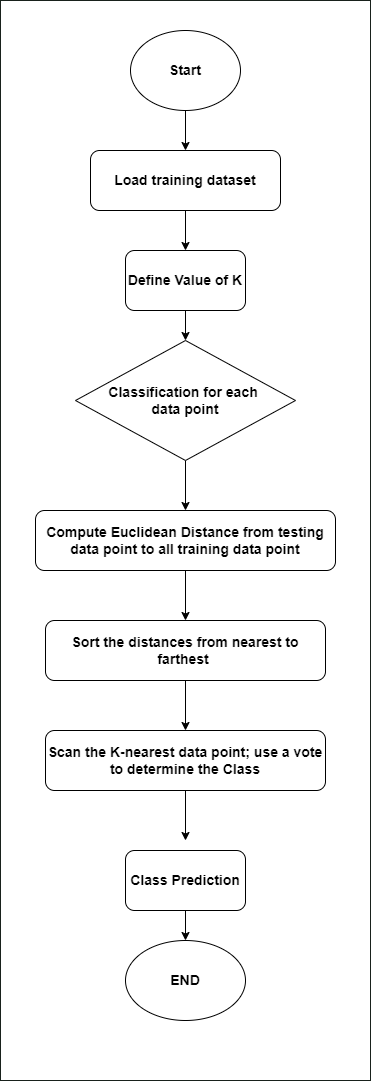
\includegraphics[width=0.5\linewidth]{KNNClassifier.png}
    \caption{KNN Flow Diagram according to steps.}
    \label{fig:enter-label}
\end{figure}




\subsection{Unit Testing and Exception Handling}
The outcomes of the unit test model are depicted in Figure.10. Unit test is developed to handle various scenarios, including handling exceptions. All the unit test which are designed and implemented for HTM classifier have been integrated into KNN classifier. During conducting the test, we have not noticed any instance failed tests. Indicating the robustness and reliability of the implemented algorithm. But there is one important thing is that the continuous testing and refinement of the model are imperative to ensure its accuracy and performance across diverse scenarios and datasets.[54]



\section{Results}
In our scenario, we utilize a data splitting method that randomly shuffles the dataset's rows, allocating a specified ratio for training and the remainder for testing. Specifically, 70\% of the data is allocated for training, while 30\% is reserved for testing. The method returns the training and testing datasets as separate arrays. 
The reported accuracy values represent the model's prediction accuracy at various values of k when tested with randomly generated test data. These accuracy percentages provide insights into the performance of our model under different configurations of the k-Nearest Neighbors algorithm.


\begin{table}
    \centering
    \begin{tabular}{|c|c|c|c|c|c|c|c|c|}
    \hline
       
        K  & Accuracy & \multicolumn{7}{c}{Random Generated Test Data Accuracy in Percentage}\\
           \hline
          & (1) & (2) & (3) & (4) & (5) & (6) & (7) & (8)\\
                     \hline
        1 & 100 & 90.9 & 90.9  & 90.9 & 90.9 & 90.9 & 90.9 & 100\\
            \hline
        2 & 100 & 100 & 90.9 & 90.9 & 90.9 & 90.9 & 90.9 & 100\\
            \hline
        3 & 100 & 100 & 100 & 100 & 100 & 90.9 & 90.9 & 100\\
            \hline
        4 & 90.9 & 100 & 100 & 90.9 & 90.9 & 90.9 & 90.9 & 100\\
            \hline
        5 & 100 & 100 & 100 & 90.9 & 100 & 90.9 & 90.9 & 100\\
             \hline
             \
    \end{tabular}
    
    \caption{Accuracy of the KNN Classifier for different value of K for different testing Data}
    \label{tab:my_label}
\end{table}


The analysis presented in Table 1 suggests that the optimal value of k for the k-Nearest Neighbors (k-NN) classifier, when applied to a dataset with three classes, is k=3. Here's a breakdown of the findings:
\begin{enumerate}
    \item \textbf{K=1, 2, and 4:} When the model relies solely on the single nearest neighbor (k=1) or a small number of nearest neighbors (k=2, 4), the accuracy tends to hover around 90.9\%. This indicates that the classifier may be prone to misclassifications or inconsistencies when considering a small number of neighbors, leading to accuracy fluctuations.

\item \textbf{K=3:} At k=3, the accuracy consistently remains around 100\% for most randomly generated testing data splits from the dataset. This suggests that considering three nearest neighbors leads to more stable and reliable predictions, resulting in higher accuracy across various testing scenarios.
\item \textbf{K=5:} While the accuracy at k=5 is also reported as 100\%, it is noted that there are instances where the accuracy drops to 90.9\%. This indicates some variability in performance compared to k=3, where the accuracy remains consistently high.
    
\end{enumerate}


Based on these observations, it's reasonable to conclude that k=3 appears to be the optimal choice for the k-NN classifier with this dataset.

\begin{figure}
    \centering
    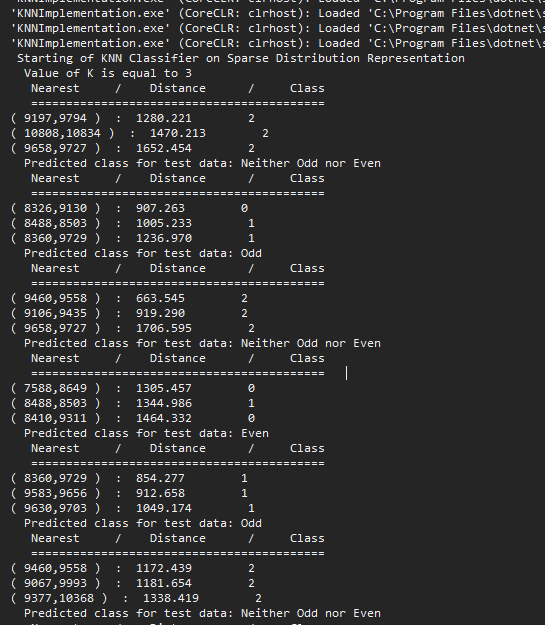
\includegraphics[width=1.0\linewidth]{Picture1.png}
    \caption{Predicted Result displayed on output window(A)}
    \label{fig :enter-label}
\end{figure}

Figures 8 \& 9 display the output window presenting the predicted results. They showcase the nearest neighbors for the test data point with a value of k set to 3, along with the calculated distances and the classification of the class for that specific test data. Subsequently, the predicted class for the test data is indicated, determining whether it is even, odd, or neither based on the voting method. This process repeats for each test data point. Finally, the model's predicted accuracy is displayed at the end.

\begin{figure}
    \centering
    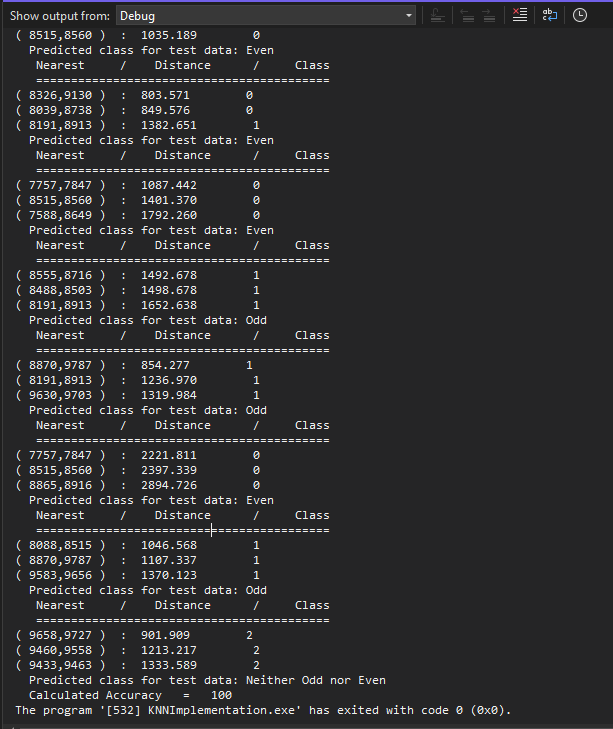
\includegraphics[width=1.0\linewidth]{Picture2.png}
    \caption{Predicted Result displayed on output window(B)}
    \label{fig:enter-label}
\end{figure}

Figure 10, depicts the unit test conducted on the KNN classifier. A random SDR is selected from the dataset, serving as the test data array to evaluate the classifier's performance. The test ensures that the predicted value by the classifier aligns with the actual class value of the test data. The KNN classifier successfully passes the unit test, as evident from the figure. Additionally, we've incorporated an exception in the unit test to accommodate varying values of K. If the value of K surpasses the length of the SDR data, the test gracefully handles this scenario.

\begin{figure}
    \centering
    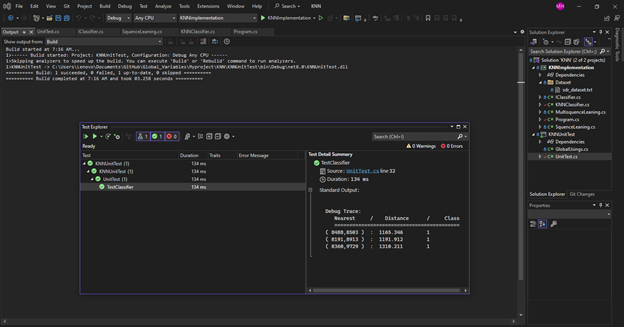
\includegraphics[width=1.0\linewidth]{Picture3.png}
    \caption{Unit Test for KNN Classifier}
    \label{fig:enter-label}
\end{figure}


\section{Application of KNN}
KNN Algorithm is utilized in different applications across different sectors, mostly in classification.[53] The common cases includes:


\subsection{Pattern Recognition}
KNN is used for the identification of specific patterns, it can be in a text. Like it predict the missing fill-in-the-blanks. This also help in solving cache which are basically handwritten numbers. So, KNN can also
to identify these patterns.


\subsection{Healthcare}
The common use of KNN is health department is prediction of chances of cancer as well as heart attacks risks.[53] The algorithm try to learn from most likely gene expressions. 

\subsection{Recommendation Engines}
When we surf on internet, the KNN algorithm can be used by the website to recommend us other additional content. This recommendation is based on user behaviour. But for larger datasets this approach is not optimal. 

\subsection{Data preprocessing}
Mostly we have a missing values in our dataset, KNN algorithm can help to determine those values. Those estimated missing values are also known as missing data imputation. 

\subsection{Finance}
The banks uses the credit card spending to predict the risk associated with the specific individual loan. As well as knn is used to determine the credit card worthiness of a loan application. So, KNN is used in a variety of economic and finance departments. As well as the other common use case is currency exchange forecasting, stock market as well as trading futures etc.  [53]



\section{Conclusion}
Firstly, we designed a straightforward KNN prototype algorithm aimed at predicting sequences. One SDR array for each sequence, we tested the model against slightly mismatched sequences, achieving the desired outcomes. To enhance the model's robustness, we compiled a comprehensive dataset consisting of SDR values corresponding to various types of sequences: even numbers, odd numbers, and decimals. This dataset enabled the model to effectively address the classification challenges posed by these sequence categories. Consequently, the model exhibits remarkable predictive accuracy. While the model consistently achieves near-perfect predictions, occasionally reaching 100\% accuracy, there were rare instances where predictions hovered around 90.9\%, still maintaining the highest level of accuracy attainable. Furthermore, we implemented unit tests to handle special cases, drawing upon the HTM Classifier for reference. These tests have yielded satisfactory results, further bolstering the reliability and performance of our model.




%
% <OR> manually copy in the resultant .bbl file
% set second argument of \begin to the number of references
% (used to reserve space for the reference number labels box)
\begin{thebibliography}{1}

\bibitem{1}
Cover, T., \& Hart, P. (1967). Nearest neighbor pattern classification. IEEE transactions on information theory, 13(1), 21-27.

\bibitem{2}
J. Z. A. L. J. W. Q. and L. S. Zhang, "An adaptive KNN algorithm based on data point density," IEEE Access, 7, 80876-80883. doi: 10.1109/ACCESS.2019.2926611, 2019.

\bibitem{3}
Guo, Gongde \& Wang, Hui \& Bell, David \& Bi, Yaxin. (2004). KNN Model-Based Approach in Classification. 

\bibitem{4}
S. A. a. J. H. Y. Cui, "Continuous Online Sequence Learning with an Unsupervised Neural Network Model," Neural Comut.,, vol. 28, pp. 2474-2504, 2016.

\bibitem{5}
Hastie, T., Tibshirani, R., and Friedman, J. (2009). The elements of statistical learning: Data mining, inference, and prediction.

\bibitem{6}
Altman, N. S. (1992). An introduction to kernel and nearest-neighbor nonparametric regression. The American Statistician, 46(3), 175-185.

\bibitem{7}
James, G., Witten, D., Hastie, T., and Tibshirani, R. (2013). An introduction to statistical learning.




%corrected

\bibitem{8}
X. L. Y. and C. Z. Yu, "Weighted K-nearest neighbor algorithm based on Gaussian kernel function," Journal of Ambient Intelligence and Humanized Computing, 11(5), 1985-1993. doi: 10.1007/s12652-019-01633-9, 2020.

\bibitem{9}
Taunk, Kashvi and De, Sanjukta and Verma, Srishti and Swetapadma, Aleena. (2019). A Brief Review of Nearest Neighbor Algorithm for Learning and Classification. 1255-1260. 10.1109/ICCS45141.2019.9065747. 


\bibitem{10}
Song Yang, Jian Huang, Ding Zhou, Hongyuan Zha, and C. Lee Giles, “Iknn:
Informative k-nearest neighbour pattern classification,” in Knowledge Discovery in Databases, (2007), pg. 248– 264.


\bibitem{11}
Han EH.., Karypis G., Kumar V.(2001) “Text Categorization Using Weight Adjusted k-Nearest Neighbour Classification”. In: Cheung D., Williams G.J., Li Q. (eds) Advances in Knowledge Discovery and Data Mining. PAKDD 2001. Lecture Notes in Computer Science, vol 2035. Springer, Berlin, Heidelberg.



\bibitem{12}
D. Wettschereck and D. Thomas G., “Locally adaptive nearest neighbour algorithms,” Adv. Neural Inf. Process. Syst., pg. 184–186, 1994.


\bibitem{13}
Bishop, C. M. (2006). Pattern recognition and machine learning.

\bibitem{14}
Zhang, Y., and Kwok, J. T. (2003). Content-based image retrieval using edge-based color histogram and adaptive similarity measure. In Proceedings of the eleventh ACM international conference on Multimedia.

\bibitem{15}
Liu, H., Yu, L., and Liu, H. (2005). Discretization: An enabling technique. Data Mining and Knowledge Discovery, 6(4), 393-423.

\bibitem{16}
Brownlee, J. (2016). Machine learning mastery with Python: Understand your data, create accurate models and work projects end-to-end.

\bibitem{17}
Mueller, A. C., and Guido, S. (2016). Introduction to machine learning with Python: A guide for data scientists.

\bibitem{18}
McKinney, W., and others. (2017). Python for data analysis: Data wrangling with Pandas, NumPy, and IPython.

\bibitem{19}
Pedregosa, F., Varoquaux, G., Gramfort, A., Michel, V., Thirion, B., Grisel, O., ... and Duchesnay, É. (2011). Scikit-learn: Machine learning in Python. Journal of Machine Learning Research, 12(Oct), 2825-2830.

\bibitem{20}
Kulkarni, A., and others. (2018). Building intelligent systems: A guide to machine learning engineering.

\bibitem{21}
Sun, Jingwen and Du, Weixing \& Shi, Niancai. (2018). A Survey of kNN Algorithm. Information Engineering and Applied Computing. 1. 10.18063/ieac.v1i1.770. 

\bibitem{22}
K. Taunk, S. De, S. Verma and A. Swetapadma, "A Brief Review of Nearest Neighbor Algorithm for Learning and Classification," 2019 International Conference on Intelligent Computing and Control Systems (ICCS), Madurai, India, 2019, pp. 1255-1260, doi: 10.1109/ICCS45141.2019.9065747.

\bibitem{23}
Komal Bharti, Prachi Shrivastava, Pradip K. Das, "Comparison of Multiple Classifiers for Audio-Visual Speaker Recognition System", 2023 International Conference on Computational Intelligence, Networks and Security (ICCINS), pp.1-6, 2023.

\bibitem{24}
Ozturk Kiyak, E.; Ghasemkhani, B.; Birant, D. High-Level K-Nearest Neighbors (HLKNN): A Supervised Machine Learning Model for Classification Analysis. Electronics 2023, 12, 3828. https://doi.org/10.3390/electronics12183828

\bibitem{25}
Zhang Z. Introduction to machine learning: k-nearest neighbors. Ann Transl Med. 2016 Jun;4(11):218. doi: 10.21037/atm.2016.03.37. PMID: 27386492; PMCID: PMC4916348.

\bibitem{26}
Cai, Y.L., Ji, D., \& Cai, D. (2010). A KNN Research Paper Classification Method Based on Shared Nearest Neighbor. NTCIR Conference on Evaluation of Information Access Technologies.

\bibitem{27}
Cover, T., Hart, P.: Nearest neighbor pattern classification. IEEE Transactions on Information Theory 13(1), 21–27 (1967)

\bibitem{28}
Goldberger, J., Roweis, S.T., Hinton, G.E., Salakhutdinov, R.: Neighbourhood components analysis. In: NIPS (2004)

\bibitem{29}
Qin, Y., Zhang, S., Zhu, X., Zhang, J., Zhang, C.: Semi-parametric optimization for missing data imputation. Applied Intelligence 27(1), 79–88 (2007)

\bibitem{30}
Weinberger, K.Q., Blitzer, J., Saul, L.K.: Distance metric learning for large margin nearest neighbor classification. In: NIPS, pp. 1473–1480 (2005)

\bibitem{31}
Wu, X., Zhang, C., Zhang, S.: Efficient mining of both positive and negative association rules. ACM Transactions on Information Systems (TOIS) 22(3), 381–405 (2004)

\bibitem{32}
Zhang, C., Zhu, X., Zhang, J., Qin, Y., Zhang, S.: GBKII: An imputation method for missing values. In: Zhou, Z.-H., Li, H., Yang, Q. (eds.) PAKDD 2007. LNCS (LNAI), vol. 4426, pp. 1080–1087. Springer, Heidelberg (2007)

\bibitem{33}
Zhang, S.: KNN-CF approach: Incorporating certainty factor to knn classification. IEEE Intelligent Informatics Bulletin 11(1), 24–33 (2010)

\bibitem{34}
Zhang, S.: Nearest neighbor selection for iteratively knn imputation. Journal of Systems and Software 85(11), 2541–2552 (2012)

\bibitem{35}
Zhu, X., Zhang, L., Huang, Z.: A sparse embedding and least variance encoding approach to hashing. IEEE Transactions on Image Processing 23(9), 3737–3750 (2014)

\bibitem{36}
D. Dobric, "“Influence of input sparsity to Hierarchical Temporal Memory Spatial Pooler Noise Robustness," 2019.

\bibitem{37}
G. K. V. K. Eui-Hong (Sam) Han, "Text Categorization Using Weight Adjusted k-Nearest Neighbor Classification," Department of Computer Science and Engineering University of Minnesota, USA, Minnesota, 1999.

\bibitem{38}
J. H. a. D. George, "“Hierarchical Temporal Memory Concepts, Theory and Terminology," Numenta, Redwood City, CA, USA, p. Available: http://www.mlanctot.info/files/papers/NumentaHTMConcepts.pdf, 2006.

\bibitem{39}
S. A. a. J. Hawkins, "Properties of Sparse Distributed Representations and their Application to Hierarchical Temporal Memory," p. Available: http://arxiv.org/abs/1503.07469, 2015.

\bibitem{40}
J. B. J. Sreedevi, "Newspaper Article Classification using MachineLearning Techniques," International Journal of Innovative Technology and Exploring Engineering, Vols. vol. 9, no. 5, pp. pp. 872-877, 2019.

\bibitem{41}
Zhu, X., Zhang, S., Jin, Z., Zhang, Z., Xu, Z.: Missing value estimation for mixed-attribute data sets. IEEE Transactions on Knowledge and Data Engineering 23(1), 110–121 (2011)

\bibitem{42}
T. M. COVER, MEMBER, IEEE, AND P. E. HART, MEMBER, IEEE, Nearest Neighbor Pattern Classification, IEEE TRANSACTIONS ON INFORMATION THEORY, VOL. IT-IS, NO. 1, JANUARY 1967

\bibitem{43}
Adeniyi, Adedayo and Wai, Zune and Yongquan, Y.. (2014). Automated Web Usage Data Mining and Recommendation System using K-Nearest Neighbor (KNN) Classification Method. Applied Computing and Informatics. 36. 10.1016/j.aci.2014.10.001. 

\bibitem{44}
M A Mukid, T Widiharih, A Rusgiyono, A Prahutama, Credit scoring analysis using weighted k nearest neighbor, OP Conf. Series: Journal of Physics: Conf. doi:10.1088/1742-6596/1025/1/012114

\bibitem{45}
Liberti, Leo \& Lavor, Carlile \& Maculan, Nelson \& Mucherino, Antonio. (2012). Euclidean Distance Geometry and Applications. SIAM Review. 56. 10.1137/120875909. 

\bibitem{46}
Suwanda, R \& Syahputra, Zulfahmi \& Zamzami, Elviawaty. (2020). Analysis of Euclidean Distance and Manhattan Distance in the K-Means Algorithm for Variations Number of Centroid K. Journal of Physics: Conference Series. 1566. 012058. 10.1088/1742-6596/1566/1/012058. 

\bibitem{47}
Lu, Binbin \& Charlton, Martin \& Brunsdon, Chris \& Harris, Paul. (2015). The Minkowski approach for choosing the distance metric in geographically weighted regression. International Journal of Geographical Information Science. 30. 1-18. 10.1080/13658816.2015.1087001. 

\bibitem{48}
Bala Priya C, KDnuggets, Distance Metrics: Euclidean, Manhattan, Minkowski, https://www.kdnuggets.com/2023/03/distance-metrics-euclidean-manhattan-minkowski-oh.html


\bibitem{49}
How to Decide the Perfect Distance Metric For Your Machine Learning Model, https://www.turing.com/kb/how-to-decide-perfect-distance-metric-for-machine-learning-model

\bibitem{50}
Euclidean Distance, https://byjus.com/maths/euclidean-distance/

\bibitem{51}
Dobric, Pech, Ghita, Wennekers 2020. 2020 International Journal of Artificial Intelligence and Applications. Scaling the HTM Spatial Pooler. doi:10.5121/ijaia .2020.11407

\bibitem{52}
Dobric, Pech, Ghita, Wennekers 2020. 2020 AIS 2020 - 6th International Conference on Artificial Intelligence and Soft Computing, Helsinki. The Parallel HTM Spatial Pooler with Actor Model. https://aircconline.com/csit/csit1006.pdf, doi:10.5121/csit.2020.100606

\bibitem{53}
Imandoust, S.B. \& Bolandraftar, Mohammad. (2013). Application of K-nearest neighbor (KNN) approach for predicting economic events theoretical background. Int J Eng Res Appl. 3. 605-610. 

\bibitem{54}
Sinha, Saurabh \& Harrold, Mary. (2000). Analysis and testing of programs with exception handling constructs. Software Engineering, IEEE Transactions on. 26. 849-871. 10.1109/32.877846. 

\bibitem{55}
Bookstein, Abraham \& Kulyukin, Vladimir \& Raita, Timo. (2002). Generalized Hamming Distance. Information Retrieval. 5. 10.1023/A:1020499411651. 

\bibitem{56}
What is the k-nearest neighbors (KNN) algorithm?, https://www.ibm.com/topics/knn

\bibitem{57}
James McCaffrey, Understanding k-NN Classification Using C\#, https://learn.microsoft.com/en-us/archive/msdn-magazine/2017/december/test-run-understanding-k-nn-classification-using-csharp


\end{thebibliography}




% that's all folks
\end{document}


